\chapter{Explications techniques}
\label{sec:technique}

%% CONTIKI =================================================================
\section{Contiki}

	Afin de créer notre sonde, nous avons utilisé Contiki, notamment la Pile réseau IPv6 et les buffers cycliques.
	
	\subsection{Pile réseau de Contiki}
	
		Contiki possède trois piles réseau :
		\begin{itemize}
			\item Rime
			\item IPv4
			\item IPv6
		\end{itemize}
		Bien évidemment, celle qui nous intéresse ici est la pile IPv6. 
		
		\subsubsection{Organisation de la pile IPv6}
			
			L'implémentation de la pile réseau nous permet d'utiliser les communications avec aisance.
			
			La pile réseau se découpe en quatre couches :
			\begin{itemize}
				\item Couche réseau
				\item Couche MAC -- Medium Access Control
				\item Couche RDC -- Radio Duty Cycling
				\item Couche radio
			\end{itemize}
			
			\clearpage
			
			\begin{figure}[htp]
				\centering
				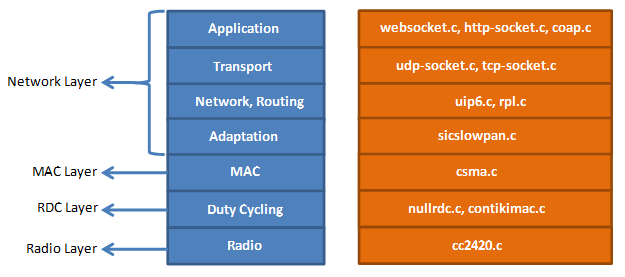
\includegraphics[width=16cm]{images/Contikinetstack}
				\caption{Organisation de la pile réseau de Contiki.}
				\label{fig:contikinetstack}
			\end{figure}
			
		\subsubsection{Packetbuf}
		
			Pour envoyer et recevoir des paquets, Contiki se base sur un buffer unique de paquets, qu'ils soient entrants ou sortants.
			Le buffer est découpé en deux parties, la première pour l'entête, et la deuxième pour les données.
			
			\begin{figure}[htp]
				\centering
				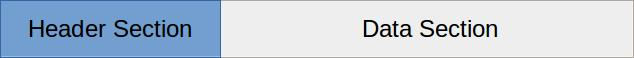
\includegraphics[width=12cm]{images/Buf.jpg}
				\caption{Découpage du buffer de paquets de Contiki.}
				\label{fig:buf}
			\end{figure}
			
			Une différence est faite entre les paquets sortants et les paquets entrants.
			
			\clearpage
			\begin{figure}[htp]
				\centering
				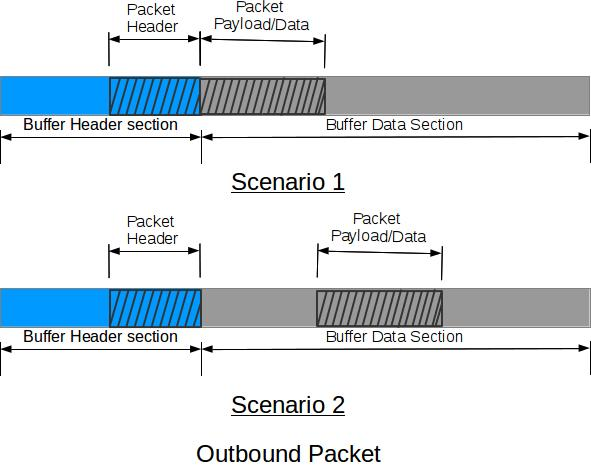
\includegraphics[width=13cm]{images/Out.jpg}
				\caption{Répartition des données pour un paquet sortant.}
				\label{fig:outbuf}
			\end{figure}
			
			
			Le buffer pour les paquets sortants permet de construire ce qu'on veut envoyer de façon structurée, avec une séparation de l'entête et des données qui permet de modifier l'un sans influer sur l'autre. 
			
			\begin{figure}[htp]
				\centering
				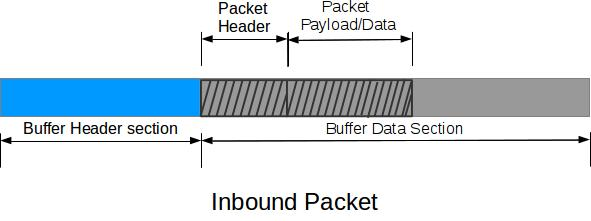
\includegraphics[width=13cm]{images/In.jpg}
				\caption{Répartition des données pour un paquet entrant.}
				\label{fig:inbuf}
			\end{figure}
			
			Le buffer pour les paquets entrant ne fait pas la différence entre entête et données, et met tout dans la partie données. Cela permet d'économiser de la puissance de calcul en évitant d'interpréter l'entête.
			Les fonctions à disposition permettent uniquement de récupérer le paquet brut.
	
	\subsection{Systèmes de stockage Contiki}
		
		Pour nos vérifications superficielles, il nous a été demandé de stocker temporairement quelques informations à propos des paquets du trafic. Nous avons considéré plusieurs options pour stocker ces informations.

		\subsubsection{Contiki Coffee file system}
%			\begin{itemize}
%				\item Expliquer comment écrire dedans
			Contiki possède plusieurs systèmes de fichiers qui implémentent l'interface de Contiki File System, dont Coffee. Coffee est utilisé sur les appareils équipés avec de la mémoire flash ou de l'EEPROM. Contiki s'occupe de l'implémentation matérielle, et Coffee fournit une API qui est similaire aux opérations sur les fichiers du langage C standard.\\
			
%				\item Expliquer pourquoi on ne l'a pas utilisé
			L'intérêt d'un système de fichier est d'envoyer d'un seul coup plusieurs données, afin de limiter le nombre de transmissions, et donc de consommer moins d'énergie. Aussi, garder les données en mémoire de façon locale permet, en cas de transmission échouée, de ne pas les perdre définitivement.
			
			Nous avons préféré nous tourner vers la mémoire volatile pour enregistrer les informations, pour avoir une solution moins lourde.
%			\end{itemize}
		\subsubsection{Volatile}
			
			La mémoire volatile de Contiki peut s'utiliser de plusieurs façons :
			\textbf{Listes}
%			\begin{itemize}
%				\item Expliquer comment écrire dedans
				The Contiki list library provides a list on which items can be placed and later retrieved. The library is used throughout Contiki for storing process lists, packet queues, neighbor lists, and various tables. List items are structures that are defined by the module that uses the list library. The only requirement is that the first item is a pointer, which the list library uses to link the items together on the list. 
				\begin{figure}[htp]
					\centering
					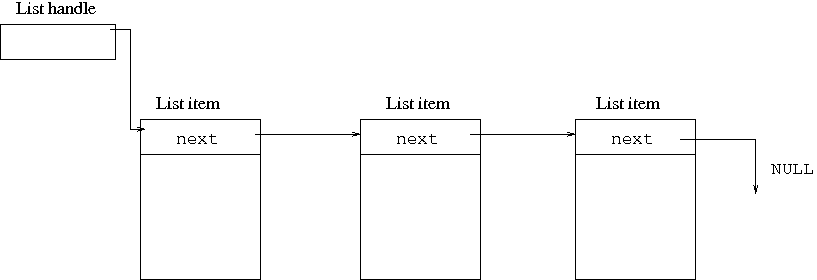
\includegraphics[width=16cm]{images/linked-list}
					\caption{Architecture d'une liste chaînée sur Contiki.}
					\label{fig:list}
				\end{figure}
				A Contiki list consists of a list handle and zero or more list items, as shown in the figure to the right. The items are linked together forming a singly linked list. The list handle is a pointer that points to the first item on the list.
				
				Items on a list are a structure where the first element is a pointer. This pointer typically is called next and is used by the list library to form the list. The last item on the list has its next pointer set to NULL. An empty list has the list handle set to NULL. 
				
%				\item Expliquer pourquoi on ne l'a pas utilisé
%			\end{itemize}
			\textbf{Buffers cycliques}
%			\begin{itemize}
%				\item Expliquer comment écrire dedans

				\begin{figure}[htp]
					\centering
					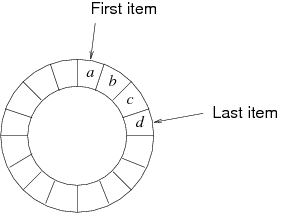
\includegraphics[width=10cm]{images/ringbuf}
					\caption{Architecture d'un buffer cyclique sur Contiki.}
					\label{fig:ringbuf}
				\end{figure}
%				\item Expliquer pourquoi on l'a utilisé
%			\end{itemize}
		
	
%% 6LoWPAN =================================================================
\section{6LoWPAN}
	\subsection{Compression des headers}
		\begin{itemize}
			\item Pourquoi compresser ?
			\item Comment ça marche ( avec images )
		\end{itemize}
	
	
	\subsection{Attaques possibles}
	\begin{itemize}
		\item Qui nous intéressent pas directement
		\begin{itemize}
			\item Attaques passives ( écoute )
			\item Brouillage des ondes
			\item Inondation de paquets
		\end{itemize}
		\item Qui nous intéressent
		\begin{itemize}
			\item Spoofing
			\item Paquets dupliqués
			\item Paquets fabriqués
			\item Sybil attack
		\end{itemize}
	\end{itemize}
	Nos possibles solutions du coup


%%% Local Variables: 
%%% mode: latex
%%% TeX-master: "isae-report-template"
%%% End: 
